\documentclass[12pt]{article}
\usepackage{graphicx} 
\usepackage{amsmath}
\usepackage{braket}
\setlength{\parindent}{0pt}
\usepackage{diffcoeff}

\usepackage{geometry}
\geometry{
    a4paper,
    left=2cm,
    right=2cm,
    top=2cm,
    bottom=2cm,
}

\title{QM Project}
\author{Nishanth S S}
\date{May 2024}

\begin{document}

\maketitle

\noindent
\textbf{Question:}
\\
\\
Imagine a harmonic oscillator potential V(x) = 
$\frac{1}{2}$m$\omega^2 x^{2}$, where we set $\omega$ = 1. We know the exact $\psi_o$. Now, we 
introduce a small perturbation v'(x) = A$e^\frac{-x^2}{2\sigma^2}$,  $\sigma = 0.25$ and A = 0.01. 
What would your choice of a trial wave function be for using the variational principle to estimate 
the ground state energy? What is the estimate for ground state energy using perturbation theory? 
With these two results in mind can you compare the exact results (numerically) with the two estimates as a function of A? 
\\

\noindent
\textbf{Solution:}
\\
\\
Using Perturbation Theory:
\\
\\
We know that, m = $\hbar = \omega$ = 1 and $\tilde{A} = (\frac{m \omega}{\pi})^\frac{1}{4}$

\[ V(x) = \frac{1}{2}m\omega^2 x^{2} + A e^{\frac{-x^2}{2\sigma^2}} \]

\[ \psi_o = \tilde{A} e^{\frac{-m \omega x^2}{2}} \]

\[ E' = \bra{\psi_o} H' \ket{\psi_o} = A\tilde{A}^2 \int e^{-x^2(m \omega + \frac{1}{2 \sigma^2})}  dx \]

\[ = A \sqrt{\frac{m \omega}{\pi}} \sqrt{\frac{\pi}{m \omega + \frac{1}{2 \sigma^2}}} \]

\[ = A \sqrt{\frac{1}{(1 + \frac{1}{2 \sigma^2})}} = A \sqrt{\frac{2 \sigma^2}{2 \sigma^2 + 1}} \]
\\

Thus, we have \[E' = A \sqrt{\frac{2 \sigma^2}{2 \sigma^2 + 1}} \]
\\
\\
\( \implies \)Total ground state energy $= \frac{\hbar \omega}{2} + E' = \frac{1}{2} + A \sqrt{\frac{2 \sigma^2}{2 \sigma^2 + 1}} $

\vspace{2 cm}

\newpage
Using Variational Principle:

\noindent
\\
Let's consider a trial function, $\psi_t = N(\tilde{A}e^{\frac{-m \omega x^2}{2}} - C_1e^{\frac{-C_2 x^2}{2}})$ where N is the normalising factor. 

\noindent
\\
We know that, $\braket{\psi_t|\psi_t} = 1$

 \[ \implies N^2 \int (\tilde{A}e^{\frac{-m \omega x^2}{2}} - C_1e^{\frac{-C_2 x^2}{2}})^2 dx = 1\]


\[ N^2 \int(\tilde{A}^2 e^{-m \omega x^2} + C_1^2 e^{-C_2 x^2} - 2\tilde{A}C_1 e^{\frac{-m \omega C_2 x^2}{2}})dx = 1\]

\[ N^2 \Big[\tilde{A}^2 \sqrt{\frac{\pi}{m \omega}} + C_1^2 \sqrt{\frac{\pi}{C_2}} - 2 \Tilde{A} C_1 \sqrt{{\frac{2 \pi}{m \omega C_2}}} \Big] = 1 \]

\begin{equation}
N^2 = \frac{1}{1 + C_1^2 \sqrt{\frac{\pi}{C_2}} - 2C_1 \pi^\frac{1}{4} \sqrt{\frac{2}{C_2}}} 
\end{equation}
\\
\\
The Hamiltonian of this system is given by, 
\[\hat{H} = -\frac{1}{2}\diff[2]{}{x} + \frac{1}{2}m\omega^2 x^{2} + A e^{\frac{-x^2}{2\sigma^2}}\]

where, Kinetic Energy = $\hat{T} =  -\frac{1}{2}\diff[2]{}{x}$ and Potential Energy = $\frac{1}{2}m\omega^2 x^{2} + A e^{\frac{-x^2}{2\sigma^2}}$
\\
\\
\\
The expectation value of the Hamiltonian gives us the average energy.

\[ \implies E = \bra{\psi_t}H\ket{\psi_t}\] 

\[E = N^2 \int (\tilde{A}e^{\frac{-m \omega x^2}{2}} - C_1e^{\frac{-C_2 x^2}{2}})( -\frac{1}{2}\diff[2]{}{x} + 
\frac{1}{2}m\omega^2 x^{2} + A e^{\frac{-x^2}{2\sigma^2}}) (\tilde{A}e^{\frac{-m \omega x^2}{2}} - C_1e^{\frac{-C_2 x^2}{2}}) dx\]

\[ E = \bra{\psi_t}\hat{T}\ket{\psi_t} + \bra{\psi_t}V\ket{\psi_t}\]
\\
\\
Let's consider the kinetic energy (the normalising factor is mentioned directly in the final result),
\[\bra{\psi_t}\hat{T}\ket{\psi_t} = \int(\tilde{A}e^{\frac{-m \omega x^2}{2}} - C_1e^{\frac{-C_2 x^2}{2}}) 
( -\frac{1}{2}\diff[2]{(\tilde{A}e^{\frac{-m \omega x^2}{2}} - C_1e^{\frac{-C_2 x^2}{2}})}{x}) dx \]

\[ = \frac{-1}{2} \int \tilde{A}e^{\frac{-m \omega x^2}{2}} \diff[2]{(\tilde{A}e^{\frac{-m \omega x^2}{2}} - C_1e^{\frac{-C_2 x^2}{2}})}{x} dx 
\quad + \quad \frac{1}{2} \int C_1e^{\frac{-C_2 x^2}{2}} \diff[2]{(\tilde{A}e^{\frac{-m \omega x^2}{2}} - C_1e^{\frac{-C_2 x^2}{2}})}{x} dx \]

\begin{multline*}   
= \frac{-\tilde{A}^2}{2} \int e^{\frac{-m \omega x^2}{2}} \diff[2]{e^{\frac{-m \omega x^2}{2}}}{x} dx \;+\;  
\frac{\tilde{A}C_1}{2} \int e^{\frac{-m \omega x^2}{2}} \diff[2]{e^{\frac{-C_2 x^2}{2}}}{x} dx \\
\;+\; \frac{\tilde{A}C_1}{2} \int e^{\frac{-C_2 x^2}{2}} \diff[2]{e^{\frac{-m \omega x^2}{2}}}{x} dx \;-\; 
\frac{C_1^2}{2} \int e^{\frac{-C_2 x^2}{2}} \diff[2]{e^{\frac{-C_2 x^2}{2}}}{x} dx 
\end{multline*} 

\newpage
\begin{multline*}
= \frac{- \tilde{A}^2}{2} \Big[(m\omega)^2 \sqrt{\frac{\pi}{m \omega}} \frac{1}{2 m \omega} - m\omega \sqrt{\frac{\pi}{m \omega}} 
\Big] \;+\; \frac{\tilde{A}C_1}{2} \Big[C_2^2 \sqrt{\frac{2 \pi}{m \omega + C_2}} \frac{1}{m \omega + C_2} - C_2 \sqrt{\frac{2 \pi}{m \omega + C_2}} \Big] \\
\\
\;+\; \frac{\tilde{A}C_1}{2} \Big[(m \omega)^2 \sqrt{\frac{2 \pi}{m \omega + C_2}} \frac{1}{m \omega + C_2} - 
m \omega \sqrt{\frac{2 \pi}{m \omega + C_2}} \Big] \;-\; \frac{C_1^2}{2} \Big[C_2^2 \sqrt{\frac{\pi}{C_2}} \frac{1}{2 C_2} - C_2 \sqrt{\frac{\pi}{C_2}} \Big]
\end{multline*}
\\
Substituting values of m,$\omega$ and $\tilde{A}$, we get 

\begin{multline*}
\bra{\psi_t}\hat{T}\ket{\psi_t} = \frac{-1}{2} \Big[\frac{\sqrt{\pi}}{2 \sqrt{\pi}} - \frac{\sqrt{\pi}}{\sqrt{\pi}} 
\Big] \;+\; \frac{C_1}{2} \Big[\frac{C_2^2}{\pi^\frac{1}{4}} \sqrt{\frac{2\pi}{1 + C_2}}\frac{1}{1 + C_2} - \frac{C_2}{\pi^\frac{1}{4}}\sqrt{\frac{2\pi}{1+C_2}} \Big] \\
\\
\;+\; \frac{C_1}{2} \Big[\frac{1}{\pi^\frac{1}{4}} \sqrt{\frac{2\pi}{1 + C_2}}\frac{1}{1 + C_2} \;-\; 
\frac{1}{\pi^\frac{1}{4}}\sqrt{\frac{2\pi}{1+C_2}} \Big] - \frac{C_1^2}{2} \Big[C_2^2 \sqrt{\frac{\pi}{C_2}}\frac{1}{2C_2} - C_2 \sqrt{\frac{\pi}{C_2}} \Big]
\end{multline*}

\begin{multline*}
= \frac{1}{4} \;+\; \frac{C_1}{2} \Big[\frac{C_2^2}{1 + C_2}\sqrt{\frac{2}{1 + C_2}} \pi^\frac{1}{4} - C_2 
\sqrt{\frac{2}{1 + C_2}} \pi^\frac{1}{4} + \sqrt{\frac{2}{1 + C_2}} \frac{\pi ^ \frac{1}{4}}{1 + C_2} \\
\\
- \sqrt{\frac{2}{1 + C_2}}\pi^\frac{1}{4} \Big] 
\;-\; \frac{C_1^2}{2} \Big[\sqrt{\frac{\pi}{C_2}} (\frac{C_2}{2} - C_2) \Big] 
\end{multline*}

\[= \frac{1}{4} + \frac{C_1}{2} \sqrt{\frac{2}{1 + C_2}} \pi^\frac{1}{4} \Big [\frac{C_2^2 - C_2 -C_2^2 +1 - 1 - C_2}{1 + C_2} 
\Big] + \frac{C_1^2 C_2}{4} \sqrt{\frac{\pi}{C_2}} \]
\\
\begin{equation}
  = N^2 \Big[\frac{1}{4} - \frac{C_1 C_2}{1 + C_2}\sqrt{\frac{2}{1 + C_2}} \pi^\frac{1}{4} + \frac{C_1^2 \sqrt{C_2 \pi}}{4} \Bigg]
\end{equation}
\\
\\
Let's consider the potential energy (the normalising factor is mentioned directly in the final result), 
\[\bra{\psi_t}V\ket{\psi_t} = \int(\tilde{A}e^{\frac{-m \omega x^2}{2}} - C_1e^{\frac{-C_2 x^2}{2}})(\frac{1}{2}m\omega^2 x^{2} + 
A e^{\frac{-x^2}{2\sigma^2}}) ((\tilde{A}e^{\frac{-m \omega x^2}{2}} - C_1e^{\frac{-C_2 x^2}{2}}) dx\]

\begin{multline*}
= \int ( \frac{\tilde{A}^2 m \omega^2 x^2}{2} e^{-m\omega x^2} + \tilde{A}^2 A e^{-x^2(m\omega + \frac{1}{2 \sigma^2})} - 
\frac{C_1 m \omega^2 \tilde{A}x^2}{2} e^{-x^2(\frac{C_2}{2} + \frac{m \omega}{2})} \\
\\
\;-\; C_1 A \tilde{A} e^{-x^2(\frac{C_2}{2} + \frac{1}{2 \sigma^2} + \frac{m \omega}{2})} - \frac{C_1 \tilde{A}m 
\omega^2 x^2}{2} e^{-x^2 (\frac{m \omega}{2} + \frac{C_2}{2})} - C_1 A \tilde{A} e^{-x^2 (\frac{C_2}{2} + \frac{1}{2 \sigma^2} + \frac{m \omega}{2})} \\
\\
\;+\; \frac{C_1^2 m \omega^2 x^2}{2} e^{-C_2 x^2} + C_1^2 A e^{-x^2(C_2 + \frac{1}{2 \sigma^2}} ) dx 
\end{multline*}
\newpage

\begin{multline*}
= \frac{\tilde{A}^2 m \omega^2}{2} \frac{\sqrt{\pi}}{2 (m\omega)^\frac{3}{2}} \;+\; \tilde{A}^2 A \sqrt{\frac{\pi}{m 
\omega + \frac{1}{2 \sigma^2}}} \;-\; \frac{2 C_1 \tilde{A} m \omega^2}{2} \frac{\sqrt{\pi}}{2 (\frac{m \omega + C_2}{2})^\frac{3}{2}} \\
\\
\;-\; 2 C_1 A \tilde{A} \sqrt{\frac{2 \pi}{C_2 + m\omega + \frac{1}{\sigma^2}}} \;+\; \frac{C_1^2 m \omega^2}{2} 
\frac{\sqrt{\pi}}{2 (C_2)^\frac{3}{2}} \;+\; C_1^2 A \sqrt{\frac{\pi}{C_2 + \frac{1}{2 \sigma^2}}}
\end{multline*}
\\
Substituting values of m,$\omega$ and $\tilde{A}$, we get 

\begin{multline*}
    \bra{\psi_t}V\ket{\psi_t} = \frac{\sqrt{\pi}}{4 \sqrt{\pi}} \;+\; \frac{A}{\sqrt{\pi}} \frac{\pi}{1 + 
    \frac{1}{2\sigma^2}} \;-\; \frac{C_1}{\pi^\frac{1}{4}} \frac{\sqrt{\pi}}{2 (\frac{1 + C_2}{2})^\frac{3}{2}} \\
    \\
    \;-\; \frac{C_1 A}{\pi^\frac{1}{4}} \sqrt{\frac{2 \pi}{C_2 + m\omega + \frac{1}{\sigma^2}}} \;+\; \frac{C_1^2}{4} 
    \frac{\sqrt{\pi}}{C_2^\frac{3}{2}} \;+\; C_1^2 A \sqrt{\frac{\pi}{C_2 + \frac{1}{2 \sigma^2}}}
\end{multline*}

\begin{equation}
    = N^2 \Big[ \frac{1}{4} \;+\; A \sqrt{\frac{2\sigma^2}{1 + 2\sigma^2}} \;-\; \frac{C_1 \pi^\frac{1}{4}}{2(\frac{1 + C_2}{2})^\frac{3}{2}} 
    \;-\; 2 C_1 A \pi^\frac{1}{4} \sqrt{\frac{2}{C_2 + 1 + \frac{1}{\sigma^2}}} \;+\; C_1^2 (\frac{\sqrt{\pi}}{4 C_2^\frac{3}{2}} 
    \;+\; A \sqrt{\frac{\pi}{C_2 + \frac{1}{2 \sigma^2}}}) \Big] \
\end{equation}
\\
\\
From equations (1),(2) and (3), we get 
\\
\\
\[ E = \bra{\psi_t}\hat{T}\ket{\psi_t} + \bra{\psi_t}V\ket{\psi_t} \]

\begin{multline*}
    = \Big[ \frac{1}{4} \;-\; \frac{C_1 C_2}{1 + C_2}\sqrt{\frac{2}{1 + C_2}} \pi^\frac{1}{4} \;+\; 
    \frac{C_1^2 \sqrt{C_2 \pi}}{4} \;+\; \frac{1}{4} \;+\; A \sqrt{\frac{2\sigma^2}{1 + 2\sigma^2}} \;-\; 
    \frac{C_1 \pi^\frac{1}{4}}{2(\frac{1 + C_2}{2})^\frac{3}{2}} \\
    \\
    \;-\; 2 C_1 A \pi^\frac{1}{4} \sqrt{\frac{2}{C_2 + 1 + \frac{1}{\sigma^2}}} \;+\; C_1^2 (\frac{\sqrt{\pi}}{4 C_2^\frac{3}{2}} 
    \;+\; A \sqrt{\frac{\pi}{C_2 + \frac{1}{2 \sigma^2}}}) \Big] N^2 
\end{multline*}

\begin{multline*}
    = \Big[ \frac{1}{2} \;+\; A \sqrt{\frac{2\sigma^2}{1 + 2\sigma^2}} \;-\; C_1 \pi^\frac{1}{4} \big( \frac{C_2 
    \sqrt{2}}{(1 + C_2)^\frac{3}{2}} + \frac{1}{2 (\frac{1 + C_2}{2})^\frac{3}{2}} \;+\; 2A \sqrt{\frac{2}{C_2 + 1 + \frac{1}{\sigma^2}}} \big) \\
    \\
    \;+\; C_1^2 \sqrt{\pi} \big(\frac{\sqrt{C_2}}{4} \;+\; \frac{1}{4 C_2^\frac{3}{2}} \;+\; \frac{A}{\sqrt{C_2 + \frac{1}{2 \sigma^2}}} \big) \Big] N^2
\end{multline*}

\newpage

\begin{equation}
\begin{split}
   E = \Big[ \frac{1}{2} \;+\; A \sqrt{\frac{2\sigma^2}{1 + 2\sigma^2}} \;-\; C_1 \pi^\frac{1}{4} \big( 
   \frac{C_2 \sqrt{2}}{(1 + C_2)^\frac{3}{2}} + \frac{1}{2 (\frac{1 + C_2}{2})^\frac{3}{2}} \;+\; 2A \sqrt{\frac{2}{C_2 + 1 + \frac{1}{\sigma^2}}} \big) 
   \\
    \\
    \;+\; C_1^2 \sqrt{\pi} \big(\frac{\sqrt{C_2}}{4} \;+\; \frac{1}{4 C_2^\frac{3}{2}} \;+\; \frac{A}{\sqrt{C_2 + 
    \frac{1}{2 \sigma^2}}}\big) \Big]  \Big[ \frac{1}{1 + C_1^2 \sqrt{\frac{\pi}{C_2}} - 2C_1 \pi^\frac{1}{4} \sqrt{\frac{2}{C_2}}} \Big]
\end{split}
\label{Energy}
\end{equation}
\\
We now fix the value of A and find the minimum value of energy by varying the values of the coefficients $C_1$ and $C_2$ in equation \ref{Energy}. 
\\
\\
We repeat this for a range of A values and compute the minimum energy values using Python.
\\
\\
Similarly, we found the energy value for a range of A through the Perturbation Theory result.
\\
\\
We then compared the minimum energy values found using the Perturbation Theory(PT) and Variational Principle(VP) 
methods with the energy values found computationally using a quantum solver in Python. 
\\
\\
The difference in the values of energy found using the quantum solver and the PT and VP methods were taken and 
plotted against the respective values of A. Below are the graphs: 
\\
\\
\begin{figure}[h]
    \centering
    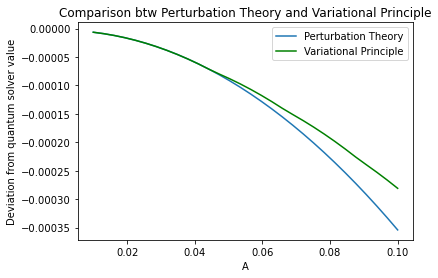
\includegraphics[width=0.8\textwidth]{Figures/Comparison btw VP and PT-1.png}
\end{figure}

\newpage

\begin{figure}[h]
    \centering
    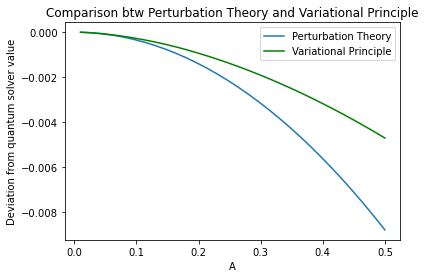
\includegraphics[width=0.8\textwidth]{Figures/Comparison btw VP and PT-2.png}
\end{figure}


From the above graphs, we can infer that VP gives a much closer value of the energy compared to PT. 

\end{document}
